\documentclass{config/apuntes}

\title{Herramientas de Programación en Bioinformática y Biología Computacional}
\author{Sandra Mingo Ramírez}
\date{2024/25}
\acronym{HPBBC}

\usepackage[all]{nowidow}
\usepackage{listing}
\usepackage{color}
\usepackage{tabularx}

\definecolor{dkgreen}{rgb}{0,0.6,0}
\definecolor{gray}{rgb}{0.5,0.5,0.5}
\definecolor{mauve}{rgb}{0.58,0,0.82}

\lstset{frame=tb,
  language=Python,
  aboveskip=3mm,
  belowskip=3mm,
  showstringspaces=false,
  columns=flexible,
  basicstyle={\small\ttfamily},
  numbers=none,
  numberstyle=\tiny\color{gray},
  keywordstyle=\color{blue},
  commentstyle=\color{dkgreen},
  stringstyle=\color{mauve},
  breaklines=true,
  breakatwhitespace=true,
  tabsize=3
}

\begin{document}

\begin{abstract}
Esta es una asignatura introductoria de los conceptos más importantes que se irán extendiendo a lo largo de todo el máster. Se divide en tres módulos: Linux, Python y Bases de Datos. 
\end{abstract}

\pagestyle{plain}

\maketitle

\tableofcontents

%02/09/24 - Eduardo Serrano (Despacho B305) eduardo.serrano@uam.es
%En los ordenadores de la EPS, al arrancarlos hay que seleccionar el segundo sistema operativo en la pantalla negra, que es el primero de Ubuntu. Después aparece una pantalla amarilla que pide usuario (mbioinf) y contraseña (2024).
 %3 módulos: introducción a linux + programación de script, introducción a python, bases de datos relacionales
%Asistencia obligatoria un 70% salvo si es demasiado inicial, en cuyo caso hay que avisar al profesor.
 %Evaluación asignatura: en las tres partes hay que hacer una práctica que cuenta un 75%. En la parte de linux se puede hacer en grupos de 3-4 personas de forma colaborativa. También hay un examen en el que hay que sacar por encima de un 4. La práctica se entrega más o menos a finales de noviembre o principios de diciembre. 
 %Se realizará detección de posibles copias mediante Turnitin, y quien copie suspenderá la asignatura y puede llegar a la suspensión del máster y de la universidad.
 %Hay que instalar linux mediante máquina virtual, cambiando el sistema operativo entero, tener particiones, linux on fly (arrancando una terminal)... La solución más chapucera vale para este curso, pero quizás para las asignaturas del resto del máster no porque hay que descargar ciertas bibliotecas, por lo que arrancarlo mediante un pendrive puede no funcionar. 
\chapter{Linux - Bash}
Todos los comandos se lanzan desde la terminal de Linux. Se pueden explorar los ficheros del árbol de directorios con un explorador que es equivalente al explorador de Windows. En cuanto se maneje con ficheros grandes, o se requieran acciones mínimas, las herramientas de la interfaz gráfica no van a ser suficientes - de ahí que tengamos que trabajar con la terminal. 

Con el comando \texttt{man comando}, \marginpar[\footnotesize man]  \ se accede al manual para buscar el comando con su nombre, descripción y posibles parámetros tanto en su versión larga como corta.

\section{Tratamiento de ficheros y directorios}
El comando \texttt{ls} \marginpar[\footnotesize ls]  \  muestra la lista de la información del directorio en el que nos encontremos. Muestra tanto los ficheros como los directorios. En Ubuntu, distingue los directorios en azul oscuro y los ficheros en verde, pero el código de colores puede cambiar en la configuración y puede no ser igual siempre, por lo que no nos deberíamos fijar en eso.  El comando se puede completar con una serie de \textbf{parámetros detrás de un guion que modifican el comportamiento del comando inicial}. \texttt{ls -l} lista el contenido del directorio con información adicional que incluye la localización del fichero, el tipo de fichero, el tamaño en bytes, los permisos, el inode y cuándo se modificó por última vez. Algunos tamaños pueden ser difíciles de leer a simple vista. Para ello, se emplea \texttt{ls -lh} que lista el contenido con el tamaño largo, de forma que indica las unidades de forma más comprensible a simple vista. De hecho, la h viene de "human".  El parámetro \texttt{-t} ordena la lista por orden de creación o modificación de más reciente a más antiguo, y \texttt{-p} añade una barra invertida a los directorios para poder distinguirlos de los ficheros. Si se escribe \texttt{-lp}, la primera columna tiene una d al inicio de todos los directorios, mientras que los ficheros tienen un guion como primer caracter. Así, todos los parámetros se pueden concatenar en \texttt{ls -lhtp}. El parámetro \texttt{ls -a} lista el contenido del directorio en el que nos encontremos, incluyendo los ficheros ocultos cuyo nombre empieza por un punto (por ejemplo, ".config"). Estos ficheros no aparecen a no ser que se añada el parámetro a para protegerlos y que no se modifiquen sin querer. "Si no quieres que alguien meta la pata, no le enseñes dónde puede meter la pata". En función de los permisos que se tenga, luego se pueden modificar esos ficheros o no. El parámetro \texttt{-i} añade un inode que será importante cuando seamos administradores, ya que es un índice que único para cada fichero que permite modificar un fichero sin modificar otro aunque se llamen igual. Aunque no se puedan tener dos ficheros en el mismo directorio que se llamen igual porque el path sería el mismo, sí puede haber dos ficheros con el mismo nombre en directorios distintos, ya que el path sería diferente, al igual que el inode.

Para crear nuevas carpetas o directorios, en el explorador es click derecho y crear nueva carpeta. \marginpar[\footnotesize mkdir] \ En la terminal, esto se traduce en el comando \texttt{mkdir nombre-carpeta-nueva}. El tamaño de un directorio no es el tamaño de lo que tenga dentro el directorio; al crear una carpeta nueva, ya tiene un tamaño de 4K, y si se tuvieran muchos ficheros muy pesados, no tiene por qué ser la suma de todos los tamaños que contenga ese directorio.

Para cambiar de directorio, se emplea el comando \texttt{cd nuevo-directorio} \marginpar[\footnotesize cd]. \ Así, el siguiente prompt incluye el directorio en el que se encuentra. Al entrar en un directorio que acabamos de crear, con el comando \texttt{ls -lht} no aparece nada, pero con \texttt{ls -lhta} aparecen dos directorios ocultos llamados "." y "..". Los dos puntos son un\textbf{ enlace al directorio anterior o padre}, de forma que con \texttt{cd ..} se va al directorio anterior. El punto simple es el \textbf{directorio actual}. 

El comando \texttt{pwd} \marginpar[\footnotesize pwd] \ muestra dónde se encuentra el \textbf{directorio actual}, es decir, el \textbf{directorio de trabajo o working directory}. El primer símbolo es una barra (/) que indica el \textbf{directorio raíz}. La virgulilla ($\sim$) lleva a la "carpeta personal", que es una traducción de \textbf{"home directory"}. Se puede mover entre directorios ya sea por path directo mediante el uso del directorio raíz o mediante el árbol del directorio con los dobles puntos o la virgulilla. 

%unix2.html
Para copiar un archivo,  \marginpar[\footnotesize cp] \ se emplea el comando \texttt{cp archivo-original archivo-nuevo}. Hay comandos que no necesitan \textbf{argumentos}, y hay comandos (como este) que sí necesitan. En este caso, requiere de dos argumentos: el archivo que se quiere copiar y el nombre que se le quiere dar a la copia. El orden es siempre \textbf{comando -parámetro argumento}. Si se quiere copiar un directorio con todo su contenido a otro directorio, es necesario añadir el parámetro \texttt{cp -r directorio-original directorio-nuevo} (r de recursivo, es decir, todo lo que haya dentro). La fecha de los ficheros copiados es de cuando se crea la copia, no la del fichero original. Solo se podrán copiar archivos en aquellos directorios en los que tengamos los permisos apropiados por el administrador. Antes de realizar el comando para copiar, la terminal realiza una serie de comprobaciones, de forma que si el nombre del archivo a copiar tiene alguna errata, salta un error al no poder realizarse el comando stat, que forma parte de las comprobaciones previas. Si se copia un directorio en otro preexistente, se copia el primer directorio en el segundo. Esto resulta en que el segundo directorio incluye los ficheros que ya estaban y un nuevo directorio nuevo dentro - no se sobreescribe todo el directorio ni se borra lo que hubiese ahí. Aun así, sigue siendo recomendable proteger los directorios sensibles añadiendo un punto antes del nombre o directamente cambiando los permisos.

Para mover un archivo, \marginpar[\footnotesize mv] \ se utiliza el comando \texttt{mv}. Se utiliza de forma similar a cp, pudiendo mover un fichero a otro directorio o al mismo con el mismo u otro nombre siempre que el nuevo directorio ya exista previamente. Si se mueve un directorio entero, se mueve con todo el contenido que tenga en el nuevo directorio, y también se le puede cambiar el nombre. 

A la hora de querer borrar, \marginpar[\footnotesize rm \\ rmdir] \ se utiliza \texttt{rm} para los archivos y \texttt{rmdir} para los directorios. Para esto último, es necesario que el directorio esté vacío. En caso de que no, se puede utilizar \texttt{rm -r directorio/} o \texttt{rm -r ./directorio/} para borrar tanto el directorio como su contenido.

En lugar de copiar un fichero y tenerlo doble, \marginpar[\footnotesize ln] \ se puede crear un link simbólico. Esto quiere decir que se crea un fichero que no tiene el contenido del fichero original (y por tanto pesa menos, solo 11 bytes), si no que redirige a ese archivo, permitiendo enlazar distintos directorios o ficheros en ordenadores en remoto. Para crear un link simbólico, el comando es \texttt{ln -s fichero-original fichero-simbolico}. Si se borra el fichero original, el enlace simbólico ya no tiene utilidad. Para borrar un enlace, se puede borrar como un fichero cualquiera con \texttt{rm}.

\begin{table}[htbp]
\begin{mdframed}[backgroundcolor=black!10]
    \centering
    Todos los ficheros tienen un nombre y una extensión, y siempre se debe escribir completo. Los directorios no llevan nunca extensión. Se recomienda no utilizar espacios en blanco en los nombres tanto de los ficheros como de los directorios porque dificulta la navegación.
    \end{mdframed}
\end{table}

\section{Mostrar contenidos en pantalla}
El comando \texttt{clear} \marginpar[\footnotesize clear] \ borra los comandos de la pantalla para dejarla vacía.

Para mostrar en pantalla el contenido de un fichero, \marginpar[\footnotesize cat] \ se puede emplear el comando \texttt{cat fichero}. No obstante, este comando no diferencia cambio de página, si no que muestra todo el contenido por pantalla aunque ocupe más. También se puede utilizar este comando con varios ficheros para que se muestren uno detrás de otro. 

Para mostrar el contenido de un fichero en la pantalla por partes, \marginpar[\footnotesize less] \ se emplea \texttt{less}. De esa forma no hay que subir y bajar en la pantalla, si no que se desplaza mediante el uso del espacio para ir por páginas enteras, enter para ir línea a línea, y la tecla q para salir (quit). 

El comando \texttt{head} \marginpar[\footnotesize head \\ tail] \ muestra en pantalla las primeras 10 líneas de un fichero por defecto. Se le puede añadir un parámetro para indicar el número de líneas que se desea ver: \texttt{head -15 fichero} muestra las primeras 15 líneas. De forma similar, \texttt{tail} muestra las últimas 10 líneas de un fichero.

\section{Buscar contenidos de ficheros}
El comando \texttt{grep} \marginpar[\footnotesize grep] \ es fundamental al utilizarse mucho con los pipes y las redirecciones (véase más abajo). Se utiliza \texttt{grep cadena-buscada fichero}, y el resultado son todas las líneas que incluyen la cadena de caracteres que se ha buscado, tanto como palabra suelta como dentro de otra palabra. Utilizando \texttt{grep -w}, se filtran aquellas líneas en las que la cadena forma palabras individuales (si se busca with, descarta within, por ejemplo). Este comando es sensible a las mayúsculas y minúsculas. Para ignorar eso, se añade el parámetro \texttt{-i}. El parámetro \texttt{-v} muestra aquellas líneas que no incluyan la cadena, \texttt{-n} incluye al inicio de cada línea el número de dicha línea, y \texttt{-c} el número de líneas que se deberían mostrar.

El comando \texttt{wc} \marginpar[\footnotesize wc] \ cuenta distintas cosas en un fichero: líneas, palabras, y bytes. Para obtener solo una de esas mediciones, se pueden añadir los parámetros \texttt{-l, -w, -c} respectivamente. Tradicionalmente, la cantidad de bytes indica la cantidad de caracteres, pero puede haber pequeñas diferencias por la codificación. Para obtener la cantidad de caracteres, se emplea \texttt{wc -m}.

%03/09
%unit3.html
\section{Redireccionamientos y pipes}
Tras ejecutar un comando, el resultado que sale en pantalla es la \textbf{salida estándar}. Sin embargo, se puede \textbf{redireccionar la salida} a otro lugar mediante el símbolo >. \marginpar[\footnotesize > \\ > >] \ Linux trata igual la salida estándar y un fichero, pero la salida estándar es la opción por defecto, por lo que nosotros debemos redireccionar la salida cuando lo queremos guardar en un fichero. Hay que tener cuidado porque si se redirecciona una salida a un fichero que ya existe, se sobreescribe el contenido del mismo. Si lo que queremos es que el contenido nuevo se añada detrás del contenido ya presente en un fichero, se deben emplear los dos símbolos > >. 

También existe un \textbf{redireccionamiento de entrada}, siendo la entrada estándar lo que se escribe por teclado. Para redireccionar la entrada, se emplea el símbolo <.  \marginpar[\footnotesize <] \ 

\begin{table}[htbp]
\begin{mdframed}[backgroundcolor=red!10]
    \centering
    \textbf{Nunca se debe emplear el mismo fichero de entrada y de salida.} Al leer un fichero, el programa va línea a línea, por lo que si se procesa la primera línea y se guarda, se sobreescribe el fichero que se usaba de entrada, afectando a la continuidad del programa.
    \end{mdframed}
\end{table}

El comando \texttt{gedit fichero} \marginpar[\footnotesize gedit] \ abre un editor de texto plano que nos permite crear un fichero y escribir su contenido. Para guardar el contenido que hemos escrito, pulsa \texttt{ctrl s} y para cerrar \texttt{ctrl q}. Aunque el editor de texto también muestre el contenido de un fichero que ya existe previamente, si el tamaño del fichero es muy grande, no es recomendable leer su contenido mediante este comando, si no mediante otros mencionados previamente como \texttt{less}.

El comando \texttt{sort} \marginpar[\footnotesize sort] \ ordena una entrada por teclado o un fichero alfanuméricamente. Si un fichero está separado en líneas, compara todos los caracteres de cada línea y empieza a ordenar por el primero. A este comando se le puede pasar directamente ficheros o se le puede redireccionar por entrada. El parámetro \texttt{-r} muestra el resultado en orden inverso, y \texttt{-u} filtra las líneas repetidas en un archivo. Para ordenar una sola parte, el parámetro \texttt{-k} permite elegir los campos a comparar.

Hay ocasiones que para obtener un resultado paso a paso,  \marginpar[\footnotesize |] \ hay que crear ficheros temporales que modificar y a los que acceder. Esto se puede evitar mediante el uso de \textbf{pipes} o barras verticales (|), que conectan los comandos antes y después del pipe. De esta forma, se omite el paso intermedio y se utiliza la salida del primer comando como entrada del segundo. 

%unix4.html
\section{Wildcards y convenciones en nombres de archivo}
Los wildcards en informática son como comodines. \marginpar[\footnotesize * \\ ?] \ Existen dos tipos: el asterisco y el símbolo de interrogación. El \textbf{asterisco} va a representar cualquier número de caracteres en el nombre de un fichero o directorio. Por ejemplo, si ponemos \texttt{prueba*}, puede resultar en el directorio pruebas y en los ficheros prueba.txt y prueba.pdf. Por el contrario, el \textbf{interrogante} representa exactamente un caracter. Así, al poner \texttt{prueba?}, el resultado será exclusivamente el directorio pruebas, pero no los ficheros.

A la hora de nombrar ficheros y directorios, se deben \textbf{evitar los símbolos especiales} tales como /, *, \& y \%. También es muy recomendable \textbf{evitar espacios entre caracteres}. En resumen, a la hora de poner un nombre a un archivo, se deberían usar solo caracteres alfanuméricos junto a barras bajas y puntos. Tradicionalmente, los nombres empiezan en minúcula y pueden terminar en un punto seguido de un grupo de letras que indican el contenido de un archivo (por ejemplo, poner al final de todos los archivos en código Python .py).

%unix5.html
\section{Seguridad del sistema de archivos (permisos de acceso)}
Cada archivo y directorio tiene \textbf{permisos de acceso asociados}, que se pueden comprobar en la primera columna al realizar \texttt{ls -lht}. Se trata de una cadena de 10 símbolos d, r, w, x, -. La d solo estará presente en primera posición e indica que se trata de un directorio. Si se trata de un fichero, en primera posición hay un guion. Los 9 símbolos restantes se agrupan en grupos de 3 en 3 y representan los \textbf{permisos del usuario, del grupo al que pertenece el usuario (y no es el usuario) y de todos los demás} respectivamente. Las opciones son:
\begin{itemize}
\item r (read): permisos de lectura y copiado de un archivo y de listar el contenido de un directorio.
\item w (write): permisos de escritura y modificado de un archivo y de crear y borrar los archivos del directorio o mover archivos a él.
\item x (execution): permisos de ejecución de un archivo cuando sea apropiado, es decir, cuando sea ejecutable. Por ejemplo, los comandos de linux como ls o mv son ficheros que se encuentra en /usr/bin/ y que se pueden ejecutar por todos a la hora de escribir esos comandos en la terminal. 
\end{itemize}
Si en lugar del caracter aparece un guion, significa que ese permiso no está dado. \marginpar[\footnotesize chmod] \ Si eres el propietario de un fichero, se pueden cambiar los permisos mediante el comando \texttt{chmod}. Para indicar a quién se le quiere cambiar el permiso, se pone u (usuario), g (grupo), o (otros), a (todos). Para quitar un permiso, se escribe un guion (-) seguido del permiso que se quiere quitar y del fichero; para dar un permiso, se escribe un más (+) y el permiso seguido del nombre del fichero. Un igual (=) expresa los permisos que se quieran. Para poner permisos diferentes, se escriben separados por comas (pero sin espacios), por ejemplo \texttt{chmod g+wx,o+w fichero}. También se puede ejecutar el comando \texttt{chmod 777 fichero} para darle todos los permisos a todos. Es importante tener en cuenta también los permisos de los directorios, ya que para poder modificar un fichero, no solo se deben tener los permisos para modificarlo, si no que a su vez debe estar en un directorio para el que se tengan los permisos para modificarlo.

\begin{table}[htbp]
\begin{mdframed}[backgroundcolor=black!10]
    \centering
    A la hora de crear ficheros, Bash proporciona al usuario autor los permisos de lectura y escritura, pero no de ejecución. Esto es importante a la hora de crear archivos ejecutables con extensión .sh.
    \end{mdframed}
\end{table}

\section{Procesos y trabajos}
Un \textbf{proceso} es un programa que se ejecuta y que recibe un \textbf{identificador (PID)} por parte del sistema operativo. Hay procesos que los lanzamos nosotros, pero hay otros que funcionan por detrás como por ejemplo buscar conexiones Wifi. 

El comando \texttt{top} muestra todos los procesos que se están llevando a cabo en tiempo real. \marginpar[\footnotesize top] \ La terminal es un proceso, y cada vez que nosotros lanzamos un proceso desde la terminal, por lo que se genera un proceso con un proceso padre (la terminal). Los procesos no pueden ejecutarse a la vez (van secuencialmente), pero el sistema operativo va gestionando los procesos y sus tiempos para que parezca que van en paralelo. Los sistemas operativos modernos pueden contener varios núcleos o kernel que permite su funcionamiento a la vez, pero dentro de cada núcleo o kernel los procesos van de forma secuencial. Para salir de top, se debe ejecutar \texttt{ctrl c}.

El comando \texttt{ps} \marginpar[\footnotesize ps] \ muestra todos los procesos que se han lanzado desde esa terminal. Añadiendo el parámetro \texttt{-ef}, se incluyen los procesos padres (lanzados por root) con el usuario que lanzó el proceso, el PID y el PID padre.

El proceso \texttt{sleep} \marginpar[\footnotesize sleep] \ está parado el tiempo que se le indique. En realidad, va a estar más tiempo debido a la gestión del tiempo del sistema operativo que va alternando distintos procesos de forma intermitente. Por ello, aunque ese proceso sí dure el tiempo determinado, el usuario tiene que esperar algo más. Si se escribe \texttt{sleep 10s \&}, se estará ejecutando de fondo (en el background), y lo que se devuelve a la terminal es el PID. Esto permite seguir utilizando la terminal para otros procesos mientras tanto. Si se va enviado un proceso en el foreground cuando se quería en el background, se puede abortar (con ctrl c) y volver a ejecutar bien o se puede detener (con ctrl z) y poner \texttt{bg} para enviarlo al background. Si por el contrario se quiere reiniciar un proceso suspendido, se pone \texttt{fg}. Esto reinicia el último proceso suspendido. Para especificar uno concreto, se debe poner su número de trabajo (no el PID): \texttt{fg \$1}. 

Para matar un proceso de forma eficiente, se puede usar el comando \texttt{kill -9} \marginpar[\footnotesize kill] \ seguido del identificador del proceso. De esta forma se asegura que también se eliminen los subprocesos generados por ese proceso y se cierren todos los recursos. Sin embargo, no es posible matar los procesos de otros usuarios.

%unix6.html
\section{Otros comandos útiles de UNIX}
\begin{itemize}
\item \textbf{df}: informa del espacio libre del sistema.

\item \textbf{du}: saca los kilobytes utilizados por cada subdirectorio. Esto puede ser útil cuando se ha superado el almacenamiento para ver qué directorio tiene más archivos. \begin{itemize}
\item -s: muestra solo un resumen
\end{itemize}

\item \textbf{gzip y gunzip}: \texttt{gzip} reduce el tamaño de un fichero utilizando el compresor Zip, resultando en un fichero con extensión .gz. \texttt{gunzip} descomprime el fichero .gz. Para esto, es necesario tener permisos de lectura.

\item \textbf{tar}: combina varios archivos en uno único que puede o no estar comprimido. \begin{itemize}
\item -c: crea un archivo.
\item -x: extrae un archivo.
\item -v: muestra el progreso de un archivo.
\item -f: nombre de archivo.
\item -t: ver el contenido del archivo.
\item -j: comprime el archivo mediante bzip2.
\item -z: comprime el archivo mediante gzip.
\item -r: añade o actualiza archivos o directorios a archivos existentes.
\item -C: directorio especificado
\item --exclude=: excluye los archivos que vayan a continuación de la orden principal. 
\end{itemize}

\item \textbf{zcat}: lee archivos de extensión .gz sin la necesidad de descomprimirlos previamente. 

\item \textbf{cut}: extrae porciones de texto de un fichero al seleccionar columnas o caracteres. \begin{itemize}
\item -d: delimitador en comillas simples (por ejemplo, \texttt{-d '|'}).
\item -f: campo o columna que se quiere extraer (\texttt{-f1} o, si se quieren varias, \texttt{-f1,2}).
\end{itemize}

\item \textbf{echo}: muestra en la salida estándar lo que se ponga a continuación. Aunque funcione directamente, es recomendable escribir las cadenas de caracteres entre comillas dobles.
 
\item \textbf{tr}: reemplaza o borra caracteres de una cadena. No admite un fichero de entrada, si no que debe venir por un pipe o utilizando el redireccionamiento de entrada. \begin{itemize}
\item -s: sustituye la secuencia que se ponga a continuación entre comillas simples con una única ocurrencia. 
\item -d: elimina los caracteres proporcionados.
\end{itemize}

\item \textbf{touch}: toca el fichero, es decir, accede a él, cambiando la fecha de acceso. Si el fichero no existe, se crea el fichero sin contenido (tamaño 0).

\item \textbf{date}: imprime en pantalla el día y la hora. Se puede personalizar la forma en la que se muestra. 

\item \textbf{file}: muestra la información de uno o varios ficheros como su codificación.

\item \textbf{stat}: muestra el archivo o el estado del archivo. También es posible acceder a la meta-información del fichero mediante el parámetro \texttt{-c} seguido de una secuencia válida. 

\item \textbf{basename y dirname}: basename elimina las partes del path en el nombre de un archivo para dejar únicamente el nombre propio. También puede eliminar el sufijo de un nombre. Por el contrario, dirname elimina el nombre del archivo para dejar únicamente el path.

\item \textbf{diff}: compara el contenido de dos ficheros y muestra las diferencias entre ambos.

\item \textbf{find}: busca en los directorios ficheros y directorios con un cierto nombre, fecha, tamaño u otro atributo que se quiera especificar. Es similar al comando \texttt{ls}, pero es más potente al buscar en todo el árbol de directorios empezando por el directorio en el que se encuentra y tener muchos filtros. Por ejemplo, para buscar todos los archivos en el directorio actual que sean de texto plano, se puede poner \texttt{find . -name "*.txt" -print}. Para buscar únicamente directorios, se debe poner \texttt{-type d} y para buscar únicamente ficheros \texttt{-type e}. También se puede filtrar por profundidad, es decir, en cuántas carpetas cuelgan los ficheros mediante \texttt{maxdepth}. Para quedarse en el directorio actual, debe ser \texttt{maxdepth 1}, y para incluir una carpeta en profundidad, \texttt{maxdepth 2}. Este parámetro se debe poner después del directorio donde empezar a buscar y antes de los demás filtros: \texttt{find . -maxdepth 1 -name "*.txt"}. 

\item \textbf{xargs}: se utiliza usualmente para combinar comandos.

\item \textbf{history}: muestra el historial de comandos.

\item \textbf{ssh}: permite acceder a un servidor de Linux remoto.

\item \textbf{nohup}: hace que haya procesos de fondo al trabajar desde un servidor remoto y que no se detengan cuando cerremos sesión.

\item \textbf{gnome-terminal}: crea una nueva terminal.
\end{itemize}

%05/09
%unit7.html
\section{Variables}
En bash, las únicas variables que se puede crear son con \textbf{cadenas de caracteres} (\texttt{x=ejemplo}). Si se pone un número, el intérprete interpreta el número como un caracter ("3" en Python). Aunque las comillas no sean necesarias, sí son recomendables (sí son obligatorias cuando hay espacios en blanco entre caracteres), y se recomienda poner las comillas dobles en lugar de las simples. Es importante \textbf{no dejar espacios} entre la variable, el igual y la cadena, ya que se interpretaría el nombre de la variable como un comando y puede dar un error. Para acceder al valor de la variable, se debe poner con un símbolo de dólar antes del nombre: \texttt{echo \$x}. Si la variable que se accede no existe, la salida estará en blanco. Las variables que creamos se borran al apagar el ordenador. Para prevenir esto, se pueden guardar las variables en el fichero de configuración .bashrc.

El sistema crea automáticamente algunas variables denominadas \textbf{variables de ambiente} cada vez que se enciende el ordenador. Esto es importante saberlo para no cambiar el valor de estas variables. Ejemplos son: \begin{itemize}
\item HOME: path completo del usuario hasta la carpeta personal o home directory.
\item USER: usuario en el que nos encontramos.
\item PATH: directorios separados por dos puntos donde el intérprete va a buscar los ficheros de los comandos si no se encuentran en el directorio de trabajo.
\item ?: guarda un 0 si el último comando ha sido correcto y un entero diferente de 0 si la última acción no ha sido ejecutada correctamente (ha dado un error). Es importante remarcar que aquí, comando verdadero es 0, mientras que en Python y otros lenguajes de programación, True es cualquier número que no sea 0.
\end{itemize}

En una terminal nueva, las variables que se habían creado no existen. \marginpar[\footnotesize export] \ Para ello, se puede usar el comando \texttt{export nombre-variable} para que terminales nuevas sí puedan acceder a las variables en ese estado. Si la variable se modifica posteriormente, si no se vuelve a exportar, la terminal nueva no tiene la actualización. A su vez, como la terminal nueva es un proceso nuevo, no le puede exportar sus variables al proceso padre.

Para evitar que una variable se modifique, \marginpar[\footnotesize readonly] \ se puede utilizar el comando \texttt{readonly nombre-variable}. 

Para guardar en una variable la salida de un comando, se debe emplear la expresión \texttt{x=\$(comando)}. Entre los paréntesis y el comando sí se pueden dejar espacios para facilitar la lectura humana. Si hay una errata en el comando y da error, la asignación a la variable no se realiza y la variable se queda sin contenido. 

Se puede crear una variable con el contenido de otras variables. Teniendo \texttt{x=3} y \texttt{y=4}, si se escribe \texttt{z=\$x+\$y}, al poner \texttt{echo \$z}, el resultado es 3+4. Esto se debe a que bash no interpreta el símbolo + como suma matemática. Para poder hacer eso, la declaración de variable y la suma se debe realizar entre doble paréntesis: \texttt{((z=x+y))}.

Para eliminar variables, se usa el comando \texttt{unset nombre-variable}. \marginpar[\footnotesize unset] \ 

\section{Scripts}
Los scripts son ficheros ejecutables de código. La extensión de estos ficheros depende del lenguaje de programación: en el caso de Python, los scripts tienen la extensión .py, y en el caso de bash, la extensión .sh. Para que un fichero se pueda ejecutar, se deben tener los \textbf{permisos de ejecución}. Además, la primera línea del código debe contener el directorio del intérprete que se debe utilizar. Tradicionalmente, los intérpretes se encuentran en /usr/bin o en /bin. Por ejemplo, la primera línea de un script de Python debe ser \texttt{\#!/usr/bin/python3} y de Bash \texttt{\#!/bin/bash}. Una vez hecho esto, desde la propia terminal se puede ejecutar el script poniendo simplemente el nombre del script.

\subsection{Variables especiales en scripts}
Es posible pasar argumentos a un script para personalizar la salida. Para asignar algo indeterminado a una variable, se emplea \texttt{\$1 - \$9}, de forma que al ejecutar el script, se deban poner los argumentos que pasará a reemplazar los huecos en ese orden. Es buena práctica que en el script los argumentos pasados por teclado se guarden en variables con nombres que tengan sentido y luego sean esas variables las que se empleen en el resto del código. De esa forma, el código queda más claro visualmente y es más fácil de modificar sin equivocaciones. Aunque quizás sea menos eficiente que utilizar el argumento donde toque en el código, así se facilita el mantenimiento del script. Por ello, nos deberíamos acostumbrar a dividir el script en tres partes: el intérprete, la declaración de variables y el código a ejecutar. Siempre que se pidan unos parámetros, se debe comprobar mediante precondiciones que se proporcionen todos los parámetros necesarios. 

Otras variables especiales son: \begin{itemize}
\item \$0: el nombre del script de bash en el que se encuentra.
\item \$\#: la cantidad de argumentos que se han pasado al script.
\item \$@: todos los argumentos que se han pasado al script.
\item \$\$: el PID del script actual.
\item HOSTNAME: nombre de la máquina en la que se está ejecutando el script. 
\item SECONDS: la cantidad de segundos desde que el script se inició. 
\item RANDOM: devuelve un número aleatorio diferente cada vez que se refiera a esto.
\item LINENO: devuelve el número de la línea actual en el script de bash.
\end{itemize}

%06/09 estudio propio + 26/09 Eduardo Serrano
%unix8.html
\section{Branching}
Las sentencias condicionales if y case ayudan a tomar decisiones en los scripts de bash. Permiten decidir si ejecutar ciertos fragmentos de código en base a ciertas condiciones.

\subsection{Expresiones condicionales}
Una expresión condicional básica hace que, si una condición es verdadera, se ejecute el siguiente código. Si la condición resulta ser falsa, entonces esas acciones no se desarrollan.
\begin{lstlisting}[language = bash]
if [ condición ]
then
	código a ejecutar; no debe estar indentado, pero es recomendable por semejanza a Python
fi
#Alternativa:
if [ condición ] ; then #el punto y coma implica salto de línea
	código
fi
\end{lstlisting}

Los posibles operadores que se pueden utilizar en la condición son muy limitados: \begin{itemize}
\item\texttt{ ! expresión}: la expresión es falsa; se invierte la condición.
\item \texttt{-z string}: la longitud de string es 0, es decir, está vacía. 
\item \texttt{string1 = string2}: string1 es igual que string2.
\item \texttt{string1 != string2}: string1 no es igual que string2.
\item \texttt{integer1 -eq integer2}: integer1 es numéricamente igual que integer2.
\item \texttt{integer1 -gt integer2}: integer1 es numéricamente mayor que integer2.
\item \texttt{integer1 -lt integer2}: integer1 es numéricamente menor que integer2.
\item \texttt{-d fichero}: el fichero existe y es un directorio.
\item \texttt{-e fichero}: el fichero existe.
\item \texttt{-r fichero}: el fichero existe y tiene el permiso de lectura.
\item \texttt{-s fichero}: el fichero existe y su tamaño es mayor que 0, es decir, no está vacío.
\item \texttt{-w fichero}: el fichero existe y tiene el permiso de escritura.
\item \texttt{-x fichero}: el fichero existe y tiene el permiso de ejecución.
\item \texttt{fichero1 -nt fichero2}: es True si fichero1 es más nuevo que fichero2.
\item \texttt{fichero1 -ot fichero2}: es True si fichero1 es más antiguo que fichero2.
\end{itemize} 

Es posible conectar varias condiciones mediante el uso de \texttt{and} y \texttt{or}. Para ello, la forma preferida es combinar condiciones individuales con los operadores \&\& para and y || para or. Otra opción sería escribir los operadores en la propia condición con \texttt{-a} para and y \texttt{-o} para or. 
\begin{lstlisting}[language = bash]
if [ condición 1 ] && [ condición 2 ]; then
	código a ejecutar
fi
\end{lstlisting}

Las expresiones condicionales pueden requerir ciertas acciones si una condición es verdadera, y otras si es falsa. Para ello, se emplea \texttt{else}:
\begin{lstlisting}[language = bash]
if [ condición ] ; then
	código a ejecutar si la condición es verdadera
else
	código a ejecutar si la condición es falsa
fi
\end{lstlisting}

En algunas ocasiones puede haber distintas condiciones que deriven en distintas acciones.
\begin{lstlisting}[language = bash]
if [ condición ]
then
	código a ejecutar
elif [ otra condición ]
then
	otro código a ejecutar
else
	código diferente
fi
\end{lstlisting}

\subsection{Bucles}
Los bucles permiten repetir una serie de comandos hasta que se llega a un objetivo. Son útiles para ahorrar en código redundante y automatizar tareas repetitivas. 
\subsubsection{For loops}
Los bucles for toman cada elemento de una lista en orden, lo asignan a una variable y se ejecuta el comando hasta que se acaben los objetos de la lista. En Bash, una lista podría ser una salida que tenga separaciones mediante blancos.
\begin{lstlisting}[language = bash]
for variable in lista ; do
	código a repetir
done
\end{lstlisting}

También es posible procesar una serie de números, pero para ello deben estar en formato C: \texttt{\{inicial..final..pasos\}}.

\subsubsection{While loops}
Los bucles while permiten repetir una lista de comandos mientras que la condición sea cierta y se detiene cuando la condición pasa a ser falsa:
\begin{lstlisting}[language = bash]
while [ condición ]
do
	código a repetir
done
\end{lstlisting}

\subsubsection{Until loops}
El bucle until es similar al while, pero repite la lista de comandos hasta que la condición sea cierta, es decir, mientras sea falsa y se detiene cuando se hace verdadera.
\begin{lstlisting}[language = bash]
until [ condición ]
do
	código a repetir
done
\end{lstlisting}

\section{Ejercicio: Copia de seguridad}
Crea un script de Bash que busque y copie en un directorio backup unos ficheros que se pasen al script.

\begin{lstlisting}[language = bash]
#! /usr/bin/bash
#Buscar y copiar en directorio backup unos ficheros

FILEIN=$1
INDIR="."
OUTDIR="./backup"

if [ $# -eq "1" ]; then
	
	#Crear directorio de salida si no existe
	if ! [ -e $OUTDIR ]; then
		mkdir $OUTDIR
	fi
	
	if ! [ -r $FILEIN ]; then
		echo "El fichero de entrada no tiene permisos de lectura"
	fi
	
	#Leer fichero y guardar en lista su contenido
	LISTA=$( cat $FILEIN )
	
	#Procesar lista: buscar fichero y copiar
	for file in $LISTA; do
		FILEPATH=$( find $INDIR -name $file )
		
		if [ -r $FILEPATH ]; then
			if [ -e $OUTDIR/$file ]; then
				rm $OUTDIR/$file
			fi
			cp $FILEPATH $OUTDIR/$file
		elif [ -z $FILEPATH ]; then
			echo "El fichero $file no existe"
		else
			echo "El fichero $file no tiene permisos de lectura"
		fi
	done
else
	echo "Falta un parámetro"
fi
\end{lstlisting}
%04/09 - Oscar Delgado - LE GUSTAN NOMBRES COMPLETOS DE VARIABLES !!!
\chapter{Programación en Python}
Los lenguajes de programación son la forma de comunicarnos con los ordenadores. Algunos lenguajes tienen bajo nivel de abstracción que trabajan en binario y por ello son más similares al propio sistema. Por otro lado, están los lenguajes de alto nivel de abstracción que son más cercanos al idioma humano. Python es el lenguaje con el mejor \textbf{balance entre potencia y simplicidad}. 

La máquina ejecuta un programa ejecutable (.exe), que está escrito en ensamblador, el lenguaje del ordenador. Para algunos lenguajes de programación, se requiere de un compilador para que genere a partir de nuestro código un ejecutable que entienda la máquina, como por ejemplo C. En el caso de Python, lo que requiere es un \textbf{intérprete}, que genera a tiempo real las instrucciones del ordenador para ejecutar nuestro código. El intérprete solía ser más lento que el compilador al tener que estar traduciendo a tiempo real el código. No obstante, a día de hoy, Python puede alcanzar un 90\% del tiempo que tardaría un programa escrito en C en ejecutarse. Esto se debe a que hay problemas paralelizables, es decir, que se pueden dividir en partes y realizar al mismo tiempo. El rendimiento de un programa depende de entrada-salida, es decir, la lectura de los datos que se encuentran en el disco duro, y eso depende de la tecnología del disco duro, no del lenguaje de programación. 

Python tiene un \textbf{gran soporte de librerías}, que son programas escritos por otras personas y que se pueden utilizar por los demás. Los comandos de Python se pueden escribir directamente desde la terminal (escribiendo primero \texttt{python3} y luego salir con ctrl d), pero eso no es cómodo. Es mejor crear primero un fichero fuente con extensión .py que luego pueda utilizar el intérprete. Para ello, se escribe \texttt{pico nombre.py}. Esto abre un editor de texto donde podemos escribir el código. Se guarda con ctrl s y se cierra con ctrl x. Para que el intérprete lo lea, se debe poner en la consola \texttt{python3 nombre.py}. En caso de que haya alguna errata o algún error en el código, a la hora de ejecutar el código por el intérprete se va a indicar en qué línea del código fuente se encuentra y qué problema hay. También existen\textbf{ programas o IDEs} que son entornos donde poder editar el código fuente de forma más intuitiva. Ejemplos son Visual Studio Code, PyCharm, Spider, etc. 

El código de Python se va ejecutando secuencialmente comando a comando. 

\section{Variables}
Las \textbf{variables} son contenedores donde guardar un contenido al que poder referirse mediante el nombre de la variable. El contenido puede ser desde números a cadenas de texto, lo que define el tipo de variable (el tipo de contenido que contiene una variable). En otros lenguajes, es necesario declarar una variable antes de poder usarla (se crea antes de meterle un contenido). Esto en Python no es necesario; la \textbf{creación de tipos es implícita por el intérprete en función del primer valor que se le dé a la variable}. Así, si se escribe directamente \texttt{age = 35}, el intérprete le da el tipo integer (número entero) a la variable age. Los \textbf{tipos en Python son implícitos y dinámicos} (pueden cambiar), lo que puede ser muy cómodo, pero también puede dar lugar a errores. Los tipos son:
\begin{itemize}
\item Integer: número entero
\item Float: número con decimales
\item String: cadena de caracteres, ya sean letras o números, que van entre comillas simples o dobles. Una vez que están definidas, ya no se pueden modificar.
\item Bool: booleanos, es decir, True o False.
\item List: lista
\item Tuple: tupla
\item Dictionary: diccionario
\end{itemize}

En cuanto a los nombres de las variables, no pueden contener espacios en blanco ni empezar por un número. Python es case-sensitive, por lo que hay una distinción entre mayúsculas y minúsculas. 

\section{Primeras nociones}
El comando \texttt{print} permite imprimir algo por pantalla. 

El comando \texttt{input} le pide información al usuario que debe aportar por teclado.
\begin{lstlisting}
name = input('Enter your name: ')
print('Hello, ', name)
\end{lstlisting}

Ese código está dividido en dos líneas de código. La primera línea es bloqueante, ya que le pide al usuario insertar por teclado su nombre. Una vez dado, ese nombre se asigna a la variable name que se emplea para imprimir por pantalla Hello y el nombre que se le ha insertado. 

Aunque los tipos de variables sean implícitos, se puede realizar un \textbf{casting}, es decir, especificar el tipo de la variable:
\begin{itemize}
\item str(variable): convierte en tipo string.
\item int(variable): convierte en tipo integer.
\item float(variable): convierte en tipo float.
\end{itemize}

Los comentarios en Python, marcados con \#, sirven para poner anotaciones para otras personas o nosotros mismos y que el intérprete va a omitir. Es buena práctica poner comentarios para explicar las partes del código.
\begin{lstlisting}
#Código de prueba
print('Esto es una prueba') #print
\end{lstlisting}

\section{Expresiones condicionales}
En Python, se pueden escribir condicionales: si algo es verdadero/falso, ocurre algo. Esto se hace mediante \texttt{if} y \texttt{else} y sirve para cambiar el flujo del programa o tomar decisiones.
\begin{lstlisting}
num_pensado = 4
num = input("Elige un número: ")

if num_pensado == num:
	print("Enhorabuena, has acertado")
else:
	print("Sigue intentando")
\end{lstlisting}

Si se cumple la condición del if, el código que se ejecuta es el que se encuentra indentado y se continúa sin ejecutarse el bloque else. Si no se cumple el if, el código que se ejecuta es el que se encuentra indentado tras else, y se omite el bloque del if. 

En el caso de que haya más condicionales, se puede utilizar \texttt{elif} seguido del siguiente condicional, siempre y cuando la condición sea de verdadero o falso:
\begin{lstlisting}
num_pensado = 4
num = input("Elige un número: ")

if num_pensado == num:
	print("Enhorabuena, has acertado")
elif num_pensado < num:
	print("No has acertado, el número es más bajo")
else:
	print("No has acertado, el número es más grande")
\end{lstlisting}

\subsection{Operadores condicionales}
Los operadores condicionales son aquellos que resultan en True o False. Los operadores son:
\begin{itemize}
\item x == y: x es igual a y. Un solo igual asigna el valor de una variable a otra, dos iguales comprueban si son lo mismo.
\item x != y: x no es igual a y.
\item x < y: x es menor que y.
\item x <= y: x es menor o igual que y.
\item x > y: x es mayor que y.
\item x >= y: x es mayor o igual que y. 
\end{itemize}

\subsection{Operadores lógicos}
Para poder incluir varios condicionales, se utilizan los operadores lógicos \textbf{and} y \textbf{or}. 

El operador \texttt{and} implica que las dos condiciones que se unen deben ser True para que el resultado sea True. Para el operador \texttt{or}, basta con que una condición sea True para que el resultado sea True.
\begin{table}[htbp]
	\centering
	\begin{tabularx}{0.5\textwidth}{XXcc}
	X & Y & X and Y & X or Y \\ \hline
	True & True & True & True \\
	True & False & False & True \\
	False & True & False & True \\
	False & False & False & False
	\end{tabularx}
\end{table}

\section{Bucles o loops}
Los bucles permiten repetir ciertas sentencias para ahorrar código redundante. 

\subsection{For loops}
Los for loops permiten repetir un código un \textbf{número determinado de veces}. La estructura típica de un for loop es:
\begin{lstlisting}
for variable in range(número inicial, número final, incremento):
	código que se quiere repetir
	
for variable in otra_variable:
	código a repetir
\end{lstlisting}

Es importante remarcar que el código que se quiere repetir debe estar indentado. Si no se pone número inicial, automáticamente empieza en 0. De igual forma, el incremento es 1 por defecto. El número final no está incluido. Por ello, si sólo se pone \texttt{range(número)}, se podría interpretar que se repite el bucle se repite el número indicado de veces. Por ejemplo, utilizando el ejemplo anterior, se podría escribir:
\begin{lstlisting}
num_pensado = 4

for i in range(5):
	num = input("Elige un número: ")
	if num_pensado == int(num):
		print("Enhorabuena, has acertado")
		break
	else:
		print("Sigue intentando")
\end{lstlisting}

La i es una variable que empieza en 0 y con cada iteración aumenta en uno hasta llegar a 4. Esto se hace automáticamente por el intérprete. Si se acierta el número antes, se sale del bucle mediante \texttt{break}.

\subsection{While loops}
Los bucles while se repiten un \textbf{número indeterminado de veces}. Este bucle depende de una condición:
\begin{lstlisting}
while condición:
	código que se quiere repetir
\end{lstlisting}

En estos bucles, es importante que la condición se modifique dentro del bucle para no crear un bucle infinito. 
\begin{lstlisting}
num_pensado = 4
fallo = True

while fallo == True:
	num = input("Elige un número: ")
	if num_pensado == num:
		print("Enhorabuena, has acertado")
		fallo = False
	else:
		print("Sigue intentando")
\end{lstlisting}
Así, cuando el usuario acierta el número, la variable fallo pasa a ser falsa y el bucle se interrumpe.

%06/09
\section{Cadenas o strings}
Las cadenas son cualquier secuencia de caracteres o números que se encuentran entre comillas simples o dobles. También hay cadenas vacías que no tienen ninguna secuencia entre las comillas. Las cadenas se pueden concatenar mediante el +. También se puede repetir el contenido de una cadena al multiplicarlo con las veces que se quiere repetir.
\begin{lstlisting}
'AB' + 'cd' # ABcd
'Hi' * 2 # HiHi 
\end{lstlisting}

Se puede calcular la longitud de una cadena mediante \texttt{len()}.  \marginpar[\footnotesize len] \
\begin{lstlisting}
cadena = "Hola"
len(cadena) #4
\end{lstlisting}

Para comprobar si una cadena contiene algo, se emplea el operador \texttt{in}. \marginpar[\footnotesize in \\ not in]  \ Para ver si no contiene algo, se usa \texttt{not in}. Esto realmente es una expresión booleana, ya que el resultado es verdadero o falso. 
\begin{lstlisting}
secuencia = "ATC"
if "G" in secuencia:
	print("La secuencia contiene guanina".)
else:
	print("La secuencia no contiene guanina.")
\end{lstlisting}

\subsection{F-strings}
A la hora de imprimir texto, es común alternar cadenas con valores de variables. Esto se puede hacer intercalando las cadenas entre comillas con las variables o con los denominados f-strings (format-strings). Los f-strings son expresiones con una sintaxis más fluida que permite darle formato a cadenas. Para imprimir el valor de variables, basta con poner el nombre de la variable entre llaves (\{\}). En caso de querer imprimir una llave en un f-string, se debe poner doble.
\begin{lstlisting}
variable = 1
print(f"El valor de la variable es {variable}.")
# Output: El valor de la variable es 1.
print(f"El valor de la variable es {{{variable}}}.")
# Output: El valor de la variable es {1}.
\end{lstlisting}

\subsection{Indexación y slicing}
Las cadenas se pueden indexar, es decir, referir a una posición en la misma cadena. Esto se realiza escribiendo la cadena (o la variable que contiene la cadena) seguido de la posición que se quiere entre corchetes. La primera posición es un 0, y las subsiguientes van incrementando en uno. A esto se le conoce como \textbf{indexación positiva}. 
\begin{lstlisting}
cadena = "hola"
cadena[0] #h
cadena[1] #o
cadena[2] #l
cadena[3] #a
\end{lstlisting}

La \textbf{indexación negativa} se refiere a acceder a la posición desde el final de la cadena. El último carácter es -1, y los siguientes van incrementando en 1. 
\begin{lstlisting}
cadena = "hola"
cadena[-1] #a
cadena[-2] #l
cadena[-3] #o
cadena[-4] #h
\end{lstlisting}

En algunas ocasiones, queremos acceder a un fragmento de una cadena. A esto se le conoce como \textbf{slicing}, y se emplea con las posiciones: \texttt{[primero:último:paso]}. La última posición no está incluida. Los pasos son opcionales, ya que tienen un valor por defecto de 1. Si se omite el primer valor, se empieza desde el primer caracter por defecto. Si se omite el último valor, se termina en el último caracter. Así, si se pone [:], se incluye todo el contenido.
\begin{lstlisting}
cadena = "hola"
cadena[1:3] #ol
cadena[::2] #hl
\end{lstlisting}

\subsection{Métodos de cadenas}
\begin{itemize}
\item lower(): devuelve la cadena con todas las letras en minúscula.
\item upper(): devuelve la cadena con todas las letras en mayúscula.
\item replace(s1, s2): reemplaza la primera cadena con la segunda.
\item count(x): cuenta el número de veces que se encuentra x.
\item index(x): devuelve la posición del primer x.
\item isalpha(): devuelve True si todos los caracteres de una cadena son letras.
\item eval(): evalúa la expresión matemática dentro de la cadena cuando el resultado es numérico.
\end{itemize}

\section{Estructuras de datos}
En Python hay cuatro estructuras de datos: listas, diccionarios, tuplas y conjuntos o sets. 

\subsection{Listas}
La lista es un \textbf{conjunto ordenado de objetos}. Pueden ser números, cadenas, booleanos, y se pueden mezclar los distintos tipos. El contenido de una lista se escribe entre corchetes y separando los distintos objetos por comas. 
\begin{lstlisting}
lista = [False, 1, 2, "tres"]
\end{lstlisting}

Las listas guardan algunas similitudes con las cadenas: \begin{itemize}
\item Son indexables y pueden sufrir slicing.
\item \texttt{len} muestra la cantidad de elementos que se encuentran en cadena.
\item El operador \texttt{in} muestra si la lista contiene algo.
\item Se puede concatenar listas mediante + y multiplicarlas con *.
\item Se pueden crear listas vacías con [].
\item Se puede iterar sobre ellas.
\end{itemize}
\begin{lstlisting}
codones = ['AAA', 'GCT', 'CCA']
for codon in codones:
	for nucleotido in codon:
		print(nucleotido)
\end{lstlisting}

Algunos métodos específicos para trabajar con listas son:
\begin{itemize}
\item \texttt{append(x}): añade x al final de la lista.
\item\texttt{sort()}: ordena la lista de forma alfabética si solo contiene letras y de pequeño a grande si solo contiene números. 
\item \texttt{count(x)}: devuelve el número de veces que aparece x en la lista.
\item \texttt{index(x)}: devuelve el índice del primer valor de x.
\item \texttt{reverse()}: revierte el orden de la lista.
\item \texttt{remove(x)}: elimina el primer x en la lista.
\item \texttt{pop(i)}: elimina el item en el índice i y devuelve su valor.
\item \texttt{insert(i,x)}: inserta x en el índice i de la lista.
\end{itemize}

\subsection{Diccionarios}
Los diccionarios son \textbf{conjuntos no ordenados de parejas de clave y valor}. Las claves deben ser únicas e inmutables de cadenas o números, ya que sirven para acceder al valor que tengan asignado. 
\begin{lstlisting}
dic_vacio = {} #Diccionario vacío
year ={'Enero':31, 'Febrero':28} #Diccionario de dos elementos
\end{lstlisting}

Se puede iterar sobre los diccionarios, pero el  elemento que se devuelve es la clave. Para que se devuelva el valor, se debe \textbf{indexar por la clave}:
\begin{lstlisting}
for month in year:
	print(month) # Imprime las claves
	print(year[month]) #Imprime los valores
\end{lstlisting}

Se pueden añadir o cambiar el valor de elementos de un diccionario mediante indexación de la clave. Si la clave no existe previamente en el diccionario, se crea con el valor que se le asigna. Si la clave ya existía, se actualiza su valor. Para eliminar elementos de un diccionario, se emplea \texttt{del()} y se indexa la clave que se quiere eliminar.

Se puede obtener una lista de todas las claves y de todos los valores con los métodos \texttt{.keys()} y \texttt{.values()} respectivamente. 

\section{Funciones}
Las funciones son una agrupación de líneas de código que se pueden ejecutar llamando el nombre de la funciones un número ilimitado de veces. De esa forma, las funciones permiten simplificar programas largos y mantenerlos. Además, eliminan código redundante. Es muy recomendable que las funciones se encuentren definidas antes de su llamada. Por convenio, todas las funciones se ponen en la parte superior del código, aunque sean llamadas solo al final. La estructura de una función es la siguiente:
\begin{lstlisting}
def nombre_funcion(argumento1, argumento2):
	código que ejecuta la función
\end{lstlisting}
El número de argumentos tiene que ser el mismo en la definición y en la llamada. No es necesario que los argumentos tengan el mismo nombre en la llamada y en la definición. Las \textbf{variables de la función son locales} y sólo se puede acceder a ellas dentro de la misma (en el ámbito de la función). 

La mayoría de las funciones devuelven un valor. Esto significa que una variable dentro de la función pase a estar disponible fuera de la misma. Para ello, se emplea \texttt{return}, el cual indica qué valor se devuelve. Cuando el código ejecuta un return, en ese momento termina la ejecución de la función, aunque haya más código posterior.
\begin{lstlisting}
def celsius_a_fahrenheit(temperatura_c):
	temperatura_f = temperatura_c * 9/5 + 32
	return temperatura_f
	
temp_c = 23
temp_f = celsius_a_fahrenheit(temp_c) 
#el valor de temp_c se pasa a la función y el valor de temperatura_f se le asigna a temp_f
\end{lstlisting}
Se pueden devolver varios valores en una función separándolos por comas. En la llamada, se pueden poner varias variables que se irán asignando en el mismo orden. Si alguna de las variables que se devuelven no se quieren guardar en una variable global, a la hora de asignar las variables se puede poner un guion bajo.
\begin{lstlisting}
def funcion(arg1, arg2, arg3):
	return arg3, arg2, arg1 
	
v1, v2, v3 = funcion(1, 2, 3) #v1 = 3, v2 = 2, v3 = 1
_, _, variable = funcion (1, 2, 3) # variable = 1
\end{lstlisting}
Las funciones no deberían escribirse para imprimir nada en pantalla, ya que entonces no sería reusable. Las funciones deberían ser modulares y autocompletadas: que reciban un valor y devuelvan un valor. Se puede hacer que una función imprima algún dato auxiliar en pantalla, pero esa no debería ser su función principal.

\subsection{Variables locales vs globales}
Las variables que se encuentran dentro de una función son variables locales, ya que no existen fuera del ámbito de la función. Por el contrario, variables globales están presentes en el código principal y existen en cualquier parte. Aunque se pueda tener una variable local que se llame igual a otra global sin que se afecten mutuamente, no es buena práctica hacer esto.

\subsection{Argumentos por defecto}
Es posible definir funciones que tengan argumentos por defecto. Esto hace que el argumento sea opcional, es decir, que en caso de no obtener un valor en la llamada, el argumento va a tener un valor predeterminado. Esto se utiliza en aquellas funciones en las que la mayoría de las veces un argumento tiene un valor. Así, solo en los casos excepcionales se debe indicar el valor, y en la mayoría de casos no se debe incluir en la llamada. Los parámetros opcionales se deben definir en la función siempre después de los parámetros obligatorios. 

\section{Librerías/módulos}
Muchas veces, vamos a necesitar importar librerías o módulos para nuestro código. Las librerías y los módulos son lo mismo; en informática, se solía hablar de librerías, pero en Python reciben el nombre de módulos. Para importar una librería, se emplea la siguiente estructura:
\begin{lstlisting}
import libreria
import libreria as lib
\end{lstlisting}
La diferencia entre la segunda línea y la primera es que en la primera, siempre se debe poner \texttt{libreria} cuando queramos usar una función que esté ella, mientras que en la segunda se le asigna el alias lib para no tener que escribir el nombre completo. Si solo se quiere importar una función de una librería, se puede escribir:
\begin{lstlisting}
from libreria import funcion
from libreria import funcion1, funcion2

libreria.funcion1()
\end{lstlisting}
Esto puede ser beneficioso si de una librería sólo se quiere importar una función, ya que actualmente hay librerías que ocupan mucho espacio y, dependiendo del código, puede ser ineficiente cargarla entera. 

\begin{table}[htbp]
\begin{mdframed}[backgroundcolor=black!10]
    \centering
    Un script en Python está organizado en tres bloques: la importación de librerías, la definición de funciones, y el código principal.
    \end{mdframed}
\end{table}

\subsection{Instalar nuevos módulos}
Desde la terminal, se puede instalar nuevos módulos de Python mediante el comando \texttt{pip install}. \marginpar[\footnotesize pip install]  \ Las librerías tienen su propia documentación en la que se detalla las funciones que tienen y cómo usarlas. Esta documentación puede estar disponible en internet o en un repositorio de GitHub. Hay que tener cuidado a la hora de instalar nuevos módulos, ya que pueden darse problemas de seguridad importantes. 

Las librerías tienen distintas versiones, por lo que se recomienda utilizar librerías que hayan sido actualizadas recientemente y haya mucha gente colaborando y mejorándola en el repositorio GitHub. Esto asegura que no esté anticuada y que tenga un número mínimo de errores, ya que la mayoría de errores se habrán solucionado ya por todos los usuarios. 

\subsection{Módulo random}
El módulo random cuenta con varias funciones que permiten obtener valores pseudoaleatorios. \marginpar[\footnotesize random \\ randint]  \ Por ejemplo, la función \texttt{randint()} saca un valor entero entre los valores inicial y final, ambos incluidos. 
\begin{lstlisting}
import random
print(random.randint(1, 10)) 
\end{lstlisting}

\subsection{Módulo requests}
El módulo requests permite interactuar con HTTP, es decir, con el formato de navegadores y páginas web. Probablemente lo vayamos a usar en el futuro para acceder a bases de datos biomédicas publicadas en la web. 

\subsection{Módulo sys}
El módulo sys permite acceder a algunas funciones del sistema. Por ejemplo, \texttt{sys.exit()} termina la ejecución de un script.

\section{Ficheros y directorios}
Trabajar con ficheros tiene un ciclo muy concreto: abrirlo, leerlo o escribirlo, y cerrarlo. Si se abren muchos ficheros y no se cierran, el ordenador se puede quedar sin memoria, por lo que es importante cerrarlos cuando ya no sean necesarios. 

Para \textbf{abrir un fichero} en Python, \marginpar[\footnotesize open() \\ readlines() \\ write() \\ close()]  \ se emplea \texttt{open(path/del/fichero, "modo")}. Modo hace referencia a cómo queremos abrir el fichero (el modo de lectura): para leer ("r"), escribir ("w"), leer y escribir ("rw") o append ("a"). Así, si solo queremos leer los datos de un fichero, lo abrimos con permisos de lectura y, al intentar escribir, daría un error. En la práctica, no hay diferencia entre los modos w y rw. Cuando se escribe en ficheros, se reescriben por completo; si queremos añadir texto al final del fichero, debemos usar el modo a que no sobreescribe el fichero. Para poder (sobre)escribir un fichero, se necesitan los permisos del sistema operativo para poder modificar el archivo. Para obtener las líneas que tiene el fichero, se utiliza el método \texttt{readlines()}. También se puede iterar sobre el fichero para obtener las líneas. Si queremos escribir en un fichero, se utiliza \texttt{write("contenido")}. Para cerrar un fichero una vez leído y modificado, se utiliza \texttt{close()}.
\begin{lstlisting}
fichero = open(ejemplo.txt) #el fichero se encuentra en el mismo directorio

contenido = fichero.readlines()
for line in fichero:
	print(line)
	
fichero.write("Nuevo contenido")
	
fichero.close()
\end{lstlisting}

\subsection{Ejercicio}
Escribir una función que escriba en un fichero una secuencia de ADN aleatoria de una longitud que reciba por parámetro.
\begin{lstlisting}
import random # alternativa: from random import choice

def escribe_secuencia_fichero(secuencia, nombre_fichero):
	fichero = open(nombre_fichero, "w")
	fichero.write(secuencia)
	fichero.close()

def generar_secuencia(longitud):
	bases = ["A", "T", "C", "G"] 
	secuencia_aleatoria = ""
	for i in range(longitud):
		secuencia_aleatoria += random.choice(bases)
	return secuencia_aleatoria
	
filename = "secuencia_aleatoria.txt"
num_bases = 10
secuencia = generar_secuencia(num_bases)
escribe_secuencia_fichero(secuencia, filename)
\end{lstlisting}

\section{Excepciones}
Una excepción es un \textbf{error irrecuperable}. Algunos errores en el programa son semánticos, es decir, son nuestros de programación. Estos son los peores porque aparentemente el programa funciona. Los errores irrecuperables hacen que el programa se detenga, como por ejemplo acceder a un fichero que no exista. Sabiendo que un código puede generar un error irrecuperable, se puede encapsular ese código dentro de una estructura especial:
\begin{lstlisting}
try:
	código que debe intentar
except Error: #ZeroDivisionError, PermissionError, IndexError, ...
	código que hacer entonces
\end{lstlisting}
Así, se captura la excepción y se da la oportunidad de hacer otra cosa. Para saber qué funciones pueden producir excepciones, se debe mirar la documentación, en la que se especifica también el tipo de error que se da. Se pueden dar varias excepciones con distintos errores para hacer el código más robusto.

Hay una excepción que recibe el nombre de Exception. Si se captura esta excepción, se captura cualquier tipo de error irrecuperable. El problema de esto es que aporta muy poca información de error y no se gestiona. Así, el programa no se para, pero tampoco se repara. Por tanto, hacer esto no es una buena práctica. 

Las excepciones pueden tener un else, el cual se ejecutará si no se lanza la excepción. De esa forma, no es necesario poner sys.exit(). Por último, existe la cláusula finally, la cual se ejecuta siempre, se lance o no una excepción. Esto es muy útil para cerrar ficheros (sobre todo si son grandes) y que no se queden en la memoria RAM cuando se da alguna excepción no capturada. 
\begin{lstlisting}
try:
	fichero = open("fichero.txt", "r")
except FileNotFoundError:
	print("El fichero no existe")
else:
	#código que podría fallar en algún momento
finally:
	fichero.close()
\end{lstlisting}

\section{Programación orientada a objetos}
Tradicionalmente, el código era lineal y se ejecutaba de forma lineal. La programación orientada a objetos presenta otro paradigma, ya que encapsula el código en objetos y clases para poder manipularlos directamente como si fuera un diccionario.
%10/09 - Ruth Cobos
\chapter{Bases de datos}
\section{Introducción a las bases de datos relacionales}
En cualquier empresa o laboratorio, se va a necesitar acceder a una gran cantidad de datos. Los \textbf{sistemas de manejo de los datos (DBMS por sus siglas en inglés)} permiten tener todos los datos juntos y relacionados para facilitar su acceso, estando de forma conveniente y eficiente de usar. Las bases de datos pueden ser muy largas y tocan todos los aspectos de nuestras vidas, desde las transacciones bancarias al registro de notas de la universidad. 

El uso de bases de datos tiene muchas ventajas, como tener un acceso más sencillo a los datos que desde múltiples ficheros e integrar los datos. Utilizar ficheros aislados puede conllevar a datos redundantes e inconsistentes, aislamiento de los datos, atomicidad de las actualizaciones, concurrencia de los accesos y problemas de seguridad.

Existen bases de datos relacionales, en las cuales los modelos de datos son entidad-relación. Hay otros paradigmas como jerárquicas, no relacionales o basados en objetos.

Las arquitecturas suelen ser cliente-servidor, pero también puede ser paralela, distribuida o centralizada. En esta asignatura utilizaremos PostgreSQL, que es de arquitectura cliente-servidor.

A partir de la década de 1950 se empezó a hablar del almacenamiento de datos en cintas magnéticas. A finales de 1960, se empezó a guardar los datos, pero no fue hasta 1980 cuando se creó el lenguaje SQL. En 1990 empiezan a aparecer las redes, la web y el data mining. A principios de los 2000 comenzaron XML y XQuery. En el siglo actual hay millones de datos (big data).

\section{Modelo de entidad relacional}
\subsection{Esquema entidad-relación (ER)}
El esquema o diagrama entidad-relación (ER) es básicamente un gráfico que muestra de forma sencilla cómo se modela la problemática que se quiere abordar con una base de datos. Va a estar compuesto por un conjunto de entidades que pueden tener atributos que los describas. Entre las entidades hay relaciones. En un esquema ER, los rectángulos representan las entidades, los diamantes las relaciones, las elipses los atributos, las líneas unen los atributos con las entidades y las entidades entre sí, y el subrayado indica los atributos clave primarios. 

\begin{figure}[htbp]
\centering
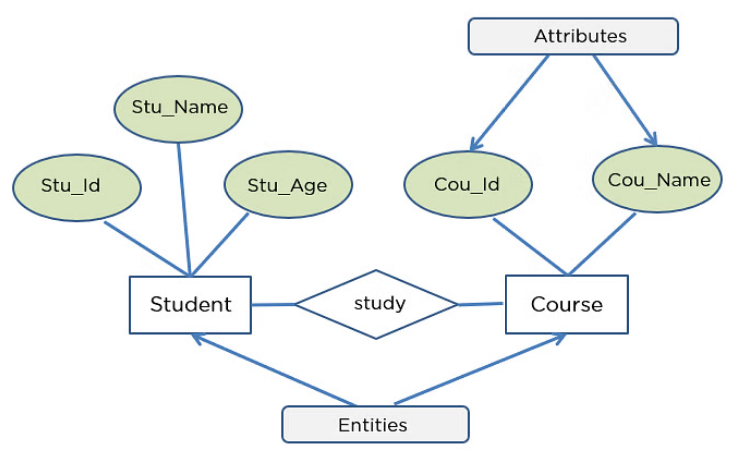
\includegraphics[width=0.5\linewidth]{figs/esquema-er.png}
\caption{Esquema ER.}
\end{figure}

Una \textbf{entidad} es un objeto o algo que pueda contener muchas instancias. Tiene atributos que le caracterizan y se deben poder distinguir de otras entidades mediante el contenido de los atributos. Normalmente, las entidades reciben un nombre en singular (por una sola palabra) y se representan con rectángulos. Las entidades débiles son aquellas cuya supervivencia depende de otra identidad.

Los \textbf{atributos} son propiedades de las entidades, y deben estar asignados a una entidad. El conjunto de valores para cada atributo se le conoce como dominio del atributo. Normalmente, los valores de los atributos son atómicos, es decir, indivisibles. 

Las \textbf{relaciones} son asociaciones entre las distintas entidades. Puede haber atributos en las relaciones. Las relaciones pueden ir también a la misma entidad en forma de bucle. En ese caso, se especifican los roles.

Es muy importante no poner en una entidad un atributo de otra entidad con la que esté relacionada.

\subsection{Claves primarias}
Una clave primaria permite identificar de manera única cada identidad. Puede ser uno o varios atributos. La clave candidata es la clave mínima primaria. Aunque puedan existir varias claves candidatas, solo una de ellas debería ser clave primaria. 

\subsection{Mapa de cardinalidades}
El mapa de cardinalidades expresa el número de entidades a los que se les puede asociar a otra entidad por una relación. Se representan por una flecha cuando es una relación individual o por una línea cuando son muchas. Hay tres cardinalidades: uno-a-uno (un cliente sólo puede pedir un préstamo, y un préstamo puede ser de un solo cliente), uno-a-muchos (un préstamo puede ser de un solo cliente, pero un cliente puede tener varios préstamos) o muchos-a-muchos (un cliente puede tener varios préstamos, y cada préstamo puede ser de varios clientes). 

\subsection{Especialización, jerarquía o generalización}
ISA se conoce como especialización, jerarquía o generalización. Viene del inglés "is a", y permite que una entidad se especialice en otras entidades. Aunque todas las entidades tengan los mismos atributos, después de la especialización las subentidades van a tener otros atributos y heredan los anteriores. Cuando en el esquema se va de arriba a abajo, se trata de una especialización, mientras que si se va de abajo a arriba se trata de una generalización. Sólo se heredan los atributos conforme se va especializando.

\subsection{Notación ER}

\begin{figure}[htbp]
\centering
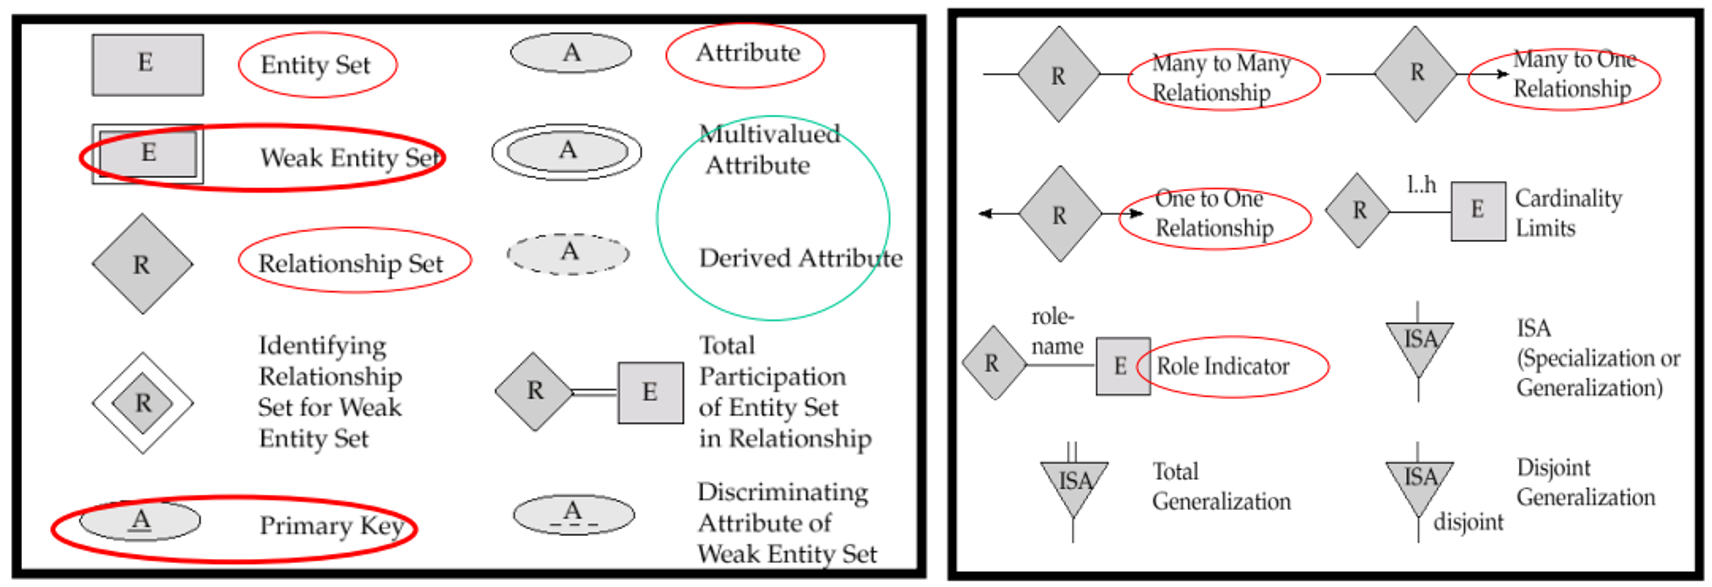
\includegraphics[width=\linewidth]{figs/notacion-er.png}
\caption{Resumen de la notación de un esquema ER. Los conceptos rodeados en rojo son los importantes. Los que están rodeados en azul no se recomiendan y los deberíamos evitar.}
\end{figure}

\subsection{Ejercicio 1: sistema de reserva de aulas para la universidad}
Vamos a hacer un sistema de reserva de salas para una universidad. Debe ser posible acceder al usuario que ha reservado cada sala, a las salas reservadas en un día concreto, o aulas concretas. Los profesores pueden reservar cualquier sala, pero los estudiantes solo pueden reservar las salas de propósito general o salas de seminario. Los usuarios se deben identificar por usuario y contraseña. 

\begin{figure}[htbp]
\centering
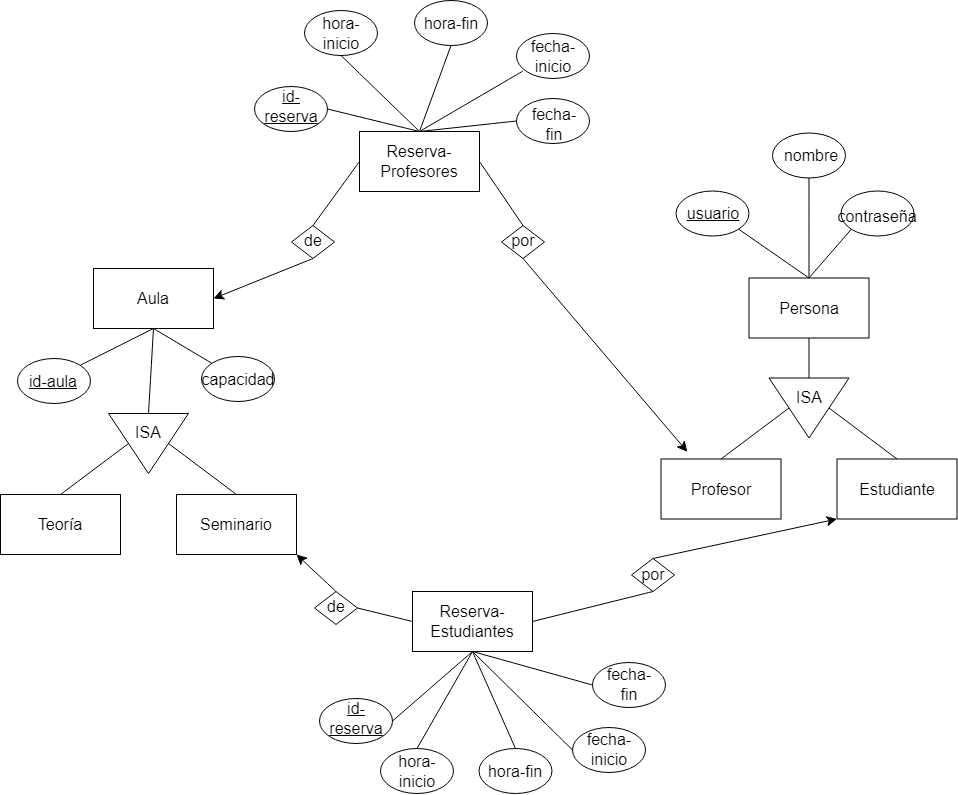
\includegraphics[width=0.7\linewidth]{figs/ejercicio-er-1.drawio.png}
\caption{Solución del ejercicio.}
\end{figure}

\subsection{Modelo relacional: esquema ER a tablas}
Desde el esquema ER, se debe convertir al modelo relacional o a un formato tabla. Para cada entidad hay una tabla única que tiene un número de columnas, que suele corresponder con los atributos, que tienen nombres únicos. Las relaciones n-n (muchos a muchos) tienen tablas separadas que consisten en las claves primarias de las dos identidades que relaciona. Las relaciones n-1 (muchos a uno) y 1-n (uno a muchos) pueden representar añadiendo un atributo extra en la parte de muchos que contenga la clave primaria de la parte uno.

A la hora de representar la especialización como tablas, hay dos opciones, y cada gestor lo hace de una manera: las especializaciones adquieren solo la clave primaria o adquiere todos los atributos de la generalización.

Los pasos para crear tablas son:
\begin{enumerate}
\item Identificar las claves primarias
\item Identificar entidades
\item Identificar los atributos redundantes de las entidades y especializar
\item Identificar relaciones n-n
\item Todas las entidades producen una tabla
\item Todas las relaciones n-n producen una tabla
\item Todas las relaciones n-1 añaden una columna a la entidad n.
\end{enumerate}

\subsection{Resumen}
El primer paso es crear el esquema ER identificando las entidades con sus atributos y relaciones, las cardinalidades y las especializaciones. Después, se debe reducir el esquema a tablas, identificando las claves primarias, entidades y relaciones n-n. Las entidades y las relaciones n-n producen una tabla. Todas las relaciones n-1 añaden columnas a la entidad de muchos.

\subsection{Ejercicio 2: gestión de mercancías}
Una empresa de gestión de mercancías desea tener almacenados los datos de sus clientes, los productos y los proveedores relacionados con los distintos pedidos que realizan los clientes. También interesa llevar un control sobre los tipos de los productos.

\begin{figure}[htbp]
\centering
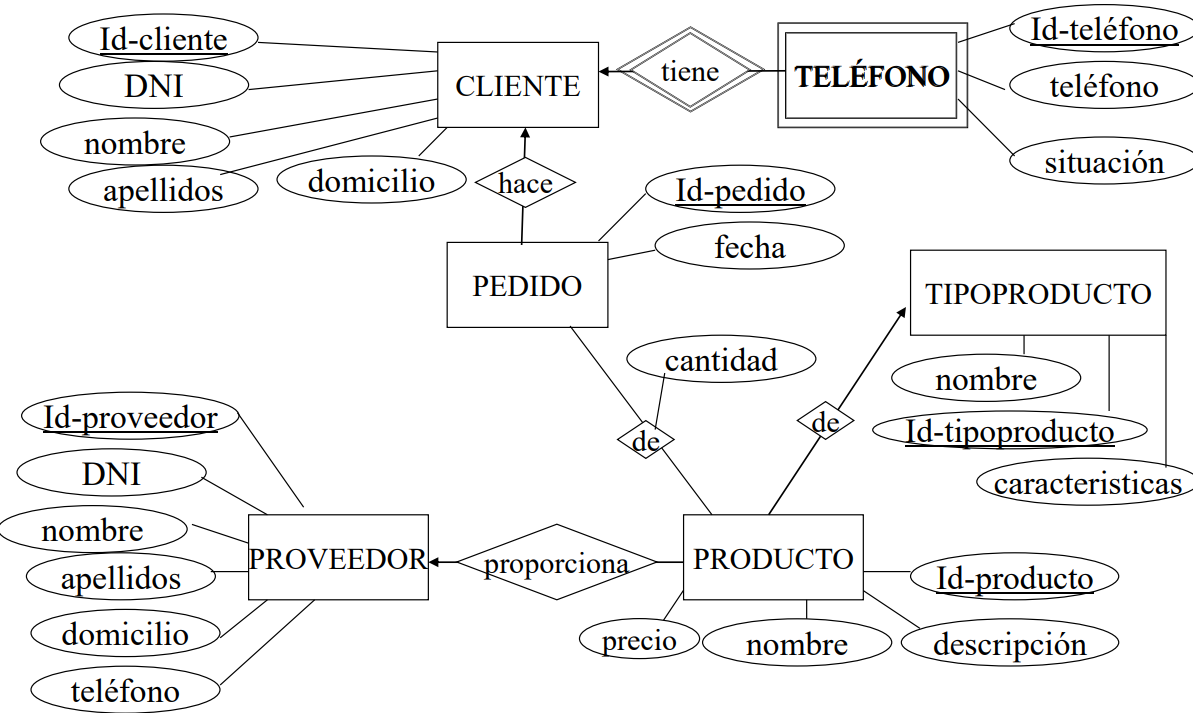
\includegraphics[width=0.7\linewidth]{figs/ejercicio-2-solucion.png}
\caption{Solución del ejercicio.}
\end{figure}

\begin{itemize}
\item Cliente (\underline{id-cliente}, DNI, nombre, apellidos, domicilio)
\item Teléfono (\underline{id-telefono}, \underline{id-cliente $\uparrow$} , telefono, situación)
\item TipoProducto (\underline{id-tipoProducto}, nombre, características)
\item Proveedor (\underline{id-proveedor}, DNI, empresa, CIF, teléfono)
\item Producto (\underline{id-producto}, id-tipoProducto $\uparrow$, id-proveedor$ \uparrow$, nombre, descripción, precio)
\item Pedido (\underline{id-pedido}, id-cliente $\uparrow$, fecha)
\item PedidoProducto / Factura (\underline{id-pedido $\uparrow$}, \underline{id-producto $\uparrow$}, cantidad) 
\end{itemize}

%17/09 - Ruth
\section{SQL: Structured Query Language}
SQL (Structured Query Language) es el lenguaje estándar de las bases de datos relacionales. Es un lenguaje declarativo que permite especificar diversos tipos de operaciones sobre estas. Es capaz de conjugar las operaciones del álgebra y el cálculo relacional con operadores adicionales, y definir así consultas para recuperar o modificar información de bases de datos, así como hacer cambios en ellas.

Los tipos de comandos en SQL se agrupan en dos categorías o sub-lenguajes:
\begin{itemize}
\item \underline{DDL (Definition Data Language)}: permite definir el esquema de bases de datos, creando relaciones (tablas), campos e índices, o modificando las definiciones existentes.
\item \underline{DML (Data Manipulation Language)}: permiten generar consultas para ordenar, filtrar y extraer datos de la base de datos, así como insertar, modificar y eliminar registros de las tablas.
\end{itemize}

Todas las queries o consultas en SQL deben terminar en punto y coma (;). Los comentarios se ponen con dos guiones.

\subsection{SQL-Data Definition Language (DDL)}
SQL-DDL proporciona comandos para definir relaciones y esquemas, borrar relaciones y modificarlas. Permite especificar las relaciones y la información de cada información: el esquema de cada relación, los valores asociados con cada atributo, restricciones de integridad, seguridad y autorización, y el conjunto de índices mantenidos en cada relación.

Los distintos tipos de datos en SQL son:
\begin{itemize}
\item \textbf{char(n):} cadena de caracteres de longitud fija n.
\item \textbf{varchar(n):} cadena de caracteres de longitud variable, siendo máximo n.
\item \textbf{integer}: número entero
\item \textbf{smallint}: pequeño entero, utiliza menos números y emplea menos memoria
\item \textbf{numeric(p,d)}: número con p dígitos y d decimales.
\item \textbf{float(n):} número flotante con al menos n dígitos.
\item \textbf{null}: valor nulo
\item \textbf{date}: muestra la fecha en formato año-mes-día
\item \textbf{time}: muestra la hora en formato hora, minuto y segundo.
\item \textbf{timestamp}: muestra la fecha y la hora
\item \textbf{interval}: periodo de tiempo
\end{itemize}

La sintaxis básica para crear una tabla y eliminarla es:
\begin{lstlisting}[language=SQL]
CREATE TABLE nombre-tabla (nombre-columna tipo-columna, nombre-columna2 tipo-columna2);
DROP TABLE nombre-tabla;
\end{lstlisting}

Se puede elegir el nombre para las tablas, pero hay algunos \textbf{nombres reservados} que no pueden adoptar: oid, tableoid, xmin, cmin, xmax, cmax, ctid.

Si un valor no se asigna a un atributo, se asigna \texttt{null} por defecto excepto si se ha predefinido un valor por defecto a la hora de crear la relación. Esto es útil porque, aunque nosotros creemos la base de datos, ésta será utilizada por muchas otras personas, de forma que los campos con valores predeterminados sirven para evitar errores.
\begin{lstlisting}[language=SQL]
CREATE SEQUENCE product_no_seq; 
CREATE TABLE product(
	product_no integer PRIMARY KEY DEFAULT nextval('product_no_seq'),
	name text, --a comment
	price numeric(10,2) DEFAULT 9.99
);
CREATE UNIQUE INDEX product_no ON product ( product_no );
\end{lstlisting}

Las \textbf{restricciones de integridad} son: 
\begin{itemize}
\item \underline{check(P)}: fuerza que el resultado de una condición sea True o Null.
\item not null: atributo que no acepta un valor nulo
\item \underline{unique (atributos)}: si se pone tras un atributo, no puede haber valores repetidos en ese atributo. También se puede escribir debajo añadiendo entre paréntesis los atributos que no se pueden repetir en combinación, es decir, se puede repetir un atributo mientras que el otro sea diferente, pero no los dos juntos. 
\item \underline{primary key}: un atributo se establece como clave primaria. Cuando se utiliza detrás de un atributo, solo se puede poner una vez. Si se quiere poner más de un campo como clave primaria, se debe poner como tupla, es decir, primary key (atributo1, atributo2). Las claves primarias no se pueden repetir, pero jamás pueden ser valores nulos. Esto lo diferencia con unique, ya que ahí sí puede haber valores nulos. 
\item \underline{foreign key references r}: se utiliza un atributo presente en otra tabla a la que se referencia. El valor de la foreign key debe existir en la tabla principal. De igual forma, no se puede borrar en la tabla original si está referenciado. Si se borra en la referencia, la tabla original no se modifica a no ser que se especifique que se borre en cascada (lo cual no se recomienda).
\end{itemize}
\begin{lstlisting}[language=SQL]
CREATE TABLE product(
	product_no integer NOT NULL,
	name text,
	id_product_type REFERENCES product_type,
	price numeric(10,2) CONSTRAINT precio_positivo CHECK (price > 0) 
);
-- Crear una restricción con nombre permite una mejor trazabilidad de errores
\end{lstlisting}

\subsection{SQL-Data Manipulation Language (DML)}
SQL define cuatro sentencias de manipulación de datos principales:
\begin{itemize}
\item \textbf{Insert:} para insertar registros en la base de datos.
\item \textbf{Update:} encargado de modificar los valores de los campos indicados, en los registros que cumplan cierta condición.
\item \textbf{Delete:} encargado de eliminar los registros de una tabla que cumplan una condición.
\item \textbf{Select:} encargado de consultar registros de la base de datos que satisfagan una condición determinada. Se utiliza para indicar al motor de datos que devuelva información de las bases de datos. Utilizado con un asterisco (*), se pide que se seleccionen todos los campos de una tabla.
\end{itemize}

A estas sentencias (salvo insert) se les debe añadir modificadores para indicar a qué tupas afectan. Ciertos modificadores (cláusulas) permiten generar criterios para definir los datos a manipular o seleccionar.
\begin{itemize}
\item \textbf{From:} establece la tabla o tablas de la/s que seleccionar los registros.
\item \textbf{Where:} condiciones que los registros a seleccionar deban cumplir.
\item \textbf{Group by:} criterio para agrupar los registros seleccionados.
\item \textbf{Having:} establece condiciones sobre datos calculados para los grupos generados por \texttt{group by}.
\item \textbf{Order by:} ordena los registros seleccionados según el orden indicado.
\end{itemize}

Se pueden insertar valores en una tabla de dos formas:
\begin{lstlisting}[language=SQL]
-- Opción 1: sin especificar los nombres de las columnas, solo los valores
INSERT INTO nombre-tabla VALUES (valores respetando el orden del create table);
-- Opción 2: especificando el nombre de los atributos
INSERT INTO nombre-tabla (atributo1, atributo2, atributo3) VALUES (valor1, valor2, null)
\end{lstlisting}

Para cambiar la estructura de una base de datos ya creada, se podría borrar y volver a crear, pero cuando ya hay datos insertados, esto no es eficiente. Para ello, se puede realizar \texttt{alter table}:
\begin{lstlisting}[language=SQL]
-- Algunos ejemplos
ALTER TABLE nombre-tabla ADD CHECK (condición);
ALTER TABLE nombre-tabla ALTER COLUMN nombre-columna SET NOT NULL;
\end{lstlisting}

%24/09 - Ruth
\subsection{Queries básicas en SQL}
A la hora de ver el contenido de una base de datos, en pgAdmin podemos seleccionar Schemes > Tables > click derecho en una tabla y View/Edit Data. Una vez ahí, se puede seleccionar todas las filas o solo las primeras 100. Esto es lo mismo que poner:
\begin{lstlisting}[language=SQL]
SELECT * FROM tabla --para seleccionar solo unas columnas, sustituir el asterisco por el nombre de las columnas
ORDER BY tabla_id ASC LIMIT 100; --DESC si se quiere descendiente
\end{lstlisting}
Para seleccionar unos datos concretos, se pueden escribir las condiciones con where. No es necesario que la columna por la que se filtre sea seleccionada. Se puede emplear en la condición el igual (=), mayor (>), menor (<) y diferente (<>):
\begin{lstlisting}[language=SQL]
SELECT title 
FROM movie 
WHERE year = 1977;
\end{lstlisting}
A la hora de querer buscar las entradas de forma alfanumérica, no se puede utilizar el igual a no ser que se escriba exactamente igual a la entrada. Para poder buscar los datos que se parezcan a una entrada que se escribe, se utiliza LIKE con los wildcards. El porcentaje indica cualquier número de caracteres, mientras que el guion bajo solo representa un carácter.
\begin{lstlisting}[language=SQL]
SELECT title 
FROM movie 
WHERE title LIKE '(S|s)tar%; -- obtendremos así Star Wars y Star Trek junto con películas que empiecen por star (en minúscula).
\end{lstlisting}
Para hacer comparaciones, pero eliminando algunas opciones, existe la opción NOT SIMILAR TO. 

El parámetro DISTINCT obtiene los datos únicos o diferentes, es decir, no repite datos repetidos. También se pueden utilizar alias, renombrando columnas para las queries mediante AS. Es importante que el filtro (where) utilice el nombre original, ya que el alias se aplicará al final: 
\begin{lstlisting}[language=SQL]
SELECT title AS titulo, year AS agno, score AS puntuacion
FROM movie
WHERE score > 9.0;
\end{lstlisting}

Para poder obtener datos de dos tablas (por ejemplo, todos los actores que han participado en una serie concreta), se necesita hacer un producto cartesiano. Esto se hace mediante los IDs de los actores y de las películas. Así, se puede realizar un filtro donde los IDs coincidan o realizar un NATURAL JOIN. Para eso último, las columnas se deben llamar igual en las dos relaciones.
\begin{lstlisting}[language=SQL]
-- Opción 1
SELECT name
FROM actor, casting
WHERE movie_id = 2 AND actor.actor_id = casting.actor_id;
-- Opción 2
SELECT name
FROM actor NATURAL JOIN casting --o NATURAL INNER JOIN para eliminar los datos nulos
WHERE movie_id = 2;
\end{lstlisting}

\subsection{Subqueries}
Las queries se pueden combinar con UNION, INTERSECT y EXCEPT. Las dos queries se escriben entre paréntesis. También es posible escribir una subquery dentro de una query para obtener mediante los operadores IN, EXISTS, ALL, ANY y BETWEEN.
\begin{lstlisting}[language=SQL]
SELECT title, name
FROM movie NATURAL JOIN casting NATURAL JOIN actor
WHERE ord = 1
AND movie_id IN (SELECT movie_id FROM casting NATURAL JOIN actor WHERE name = 'Julie Andrews')
\end{lstlisting}

Hay algunos casos en los que, si se realiza una subquery, pero en el resultado se quiere obtener algo de la subquery, se forma un bucle y la máquina tarda en procesarlo. Esto se debería evitar. 

Las vistas guardan la salida de una query de forma temporal. Posteriormente se puede utilizar como si fuese otra tabla más. La sintaxis para crear una es:
\begin{lstlisting}[language=SQL]
CREATE VIEW ranking AS
SELECT actor_id, COUNT(*) AS stars
FROM casting
WHERE ord = 1
GROUP BY actor_id;

SELECT name, stars
FROM actor NATURAL JOIN ranking
WHERE stars > 10
ORDER BY stars; 
\end{lstlisting}

\subsection{Funciones de agregación}
Una función de agregación se basa en la álgebra relacional, y puede utilizar los operadores SUM, AVG, MIN, MAX y COUNT. Estas funciones tienen sentido cuando se hacen agrupaciones mediante GROUP BY. En el SELECT, sólo se pueden encontrar agregaciones y atributos que posteriormente se encuentran en GROUP BY. Todo lo que está en el GROUP BY debe estar en el SELECT.

El parámetro HAVING permite seleccionar subgrupos. Es importante no utilizar el alias en el HAVING porque es lo último que realiza el gestor.
\begin{lstlisting}[language=SQL]
SELECT x, SUM(y) AS suma
FROM table
GROUP BY x
HAVING SUM(y) > 3;
\end{lstlisting}

\subsection{Procesamiento de queries}
Las queries se procesan en el siguiente orden:
\begin{enumerate}
\item FROM
\item WHERE
\item GROUP BY
\item HAVING
\item SELECT + alias
\item ORDER BY
\end{enumerate}

Típica query que cae todos los años: obtener la película con mayor score de cada año. Corregir un comando donde en Having se ha puesto un alias (no se debe poner). Pregunta si en el order by se puede utilizar alias.


\end{document}
